% Audited sample means from 200 distinct start/chunk pairs; each replayed twice.
% These are scalar translation magnitudes, not reconstructed trajectories.
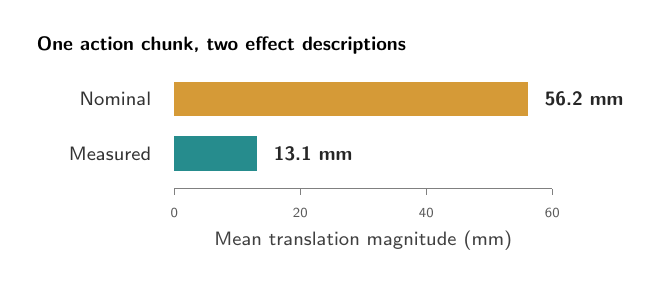
\begin{tikzpicture}[font=\sffamily\scriptsize]
\definecolor{nominalgold}{HTML}{D59A37}
\definecolor{measuredteal}{HTML}{268C8D}
\node[anchor=west,font=\sffamily\bfseries\scriptsize] at (0,2.15) {One action chunk, two effect descriptions};
\node[anchor=east,text=black!80] at (1.70,1.47) {Nominal};
\node[anchor=east,text=black!80] at (1.70,.78) {Measured};
\fill[nominalgold] (1.87,1.25) rectangle (6.365,1.69);
\fill[measuredteal] (1.87,.56) rectangle (2.922,1.00);
\node[anchor=west,font=\sffamily\bfseries\scriptsize,text=black!85] at (6.45,1.47) {56.2 mm};
\node[anchor=west,font=\sffamily\bfseries\scriptsize,text=black!85] at (3.01,.78) {13.1 mm};
\draw[black!50,thin] (1.87,.33) -- (6.67,.33);
\foreach \x/\lab in {1.87/0,3.47/20,5.07/40,6.67/60}{
  \draw[black!50,thin] (\x,.33) -- (\x,.25);
  \node[anchor=north,font=\sffamily\tiny,text=black!65] at (\x,.20) {\lab};
}
\node[anchor=north,font=\sffamily\scriptsize,text=black!75] at (4.27,-.08) {Mean translation magnitude (mm)};
\end{tikzpicture}

